\section{Pendahuluan}
\indent VPN atau Jaringan Pribadi Virtual (Virtual Private Network) membuat koneksi jaringan privat di antara
beberapa perangkat melalui internet. VPN digunakan untuk mentransmisikan data secara aman dan
anonim melalui jaringan publik. VPN bekerja dengan cara menyembunyikan alamat IP pengguna dan
mengenkripsi data sehingga tidak dapat dibaca oleh siapa pun yang tidak berwenang untuk menerimanya.
\\ \indent Salah satu service yang biasa digunakan untuk membangun sebuah jaringan VPN adalah Point to
Point Tunnel Protocol (PPTP). Sebuah koneksi PPTP terdiri dari Server dan Client. Mikrotik RouterOS
bisa difungsikan baik sebagai server maupun client atau bahkan diaktifkan keduanya bersama dalam
satu mesin yang sama. Feature ini sudah termasuk dalam package PPP sehingga anda perlu cek di
menu system package apakah paket tersebut sudah ada di router atau belum. Fungsi PPTP Client
juga sudah ada di hampir semua OS, sehingga kita bisa menggunakan Laptop/PC sebagai PPTP
Client.
\\ \indent Biasanya PPTP ini digunakan untuk jaringan yang sudah melewati multihop router (Routed Network).
Jika anda ingin menggunakan PPTP pastikan di Router anda tidak ada rule yang melakukan blocking
terhadap protocol TCP 1723 dan IP Protocol 47/GRE karena service PPTP menggunakan protocol
tersebut.


%===========================================================%

\section{Tujuan Praktikum}
Mengetahui cara menggunakan dan mengkonfigurasi VPN PPTP pada router mikrotik. Memahami penerapan dan penghubungan jaringan dengan menerapkan PPTP dengan VPN.
%===========================================================%

\section{Alat dan Bahan}
\begin{itemize}[label=$\bullet$, itemsep=-1pt, leftmargin=*]
	\item 2 buah Cloud Core Router
	\item 3 Kabel UTP (LAN)
	\item 2 buah Laptop
	\item Software Winbox
\end{itemize}
%===========================================================%

\section{Langkah-langkah Percobaan}
\textbf{gambar pada langkah-langkah di bagian ini akan diisi gambar contoh dari template dulu,
		karena nanti akan kami ganti dengan screenshot langkah-langkah kami saat praktikum}

%Langkah untuk konfigurasi Router 1
\begin{center} 
	\textbf{Konfigurasi PC 1}
\end{center}

\begin{enumerate}
	% poin 1
	\item Buka aplikasi Winbox pada PC dan lakukan hubungkan ke Router. Pastikan Login terisi “admin”,
	Klik Neighbors > Klik Refresh > Pilih Router yang ingin disambungkan > Klik Connect.
	
	\begin{figure}[H]
		\centering
		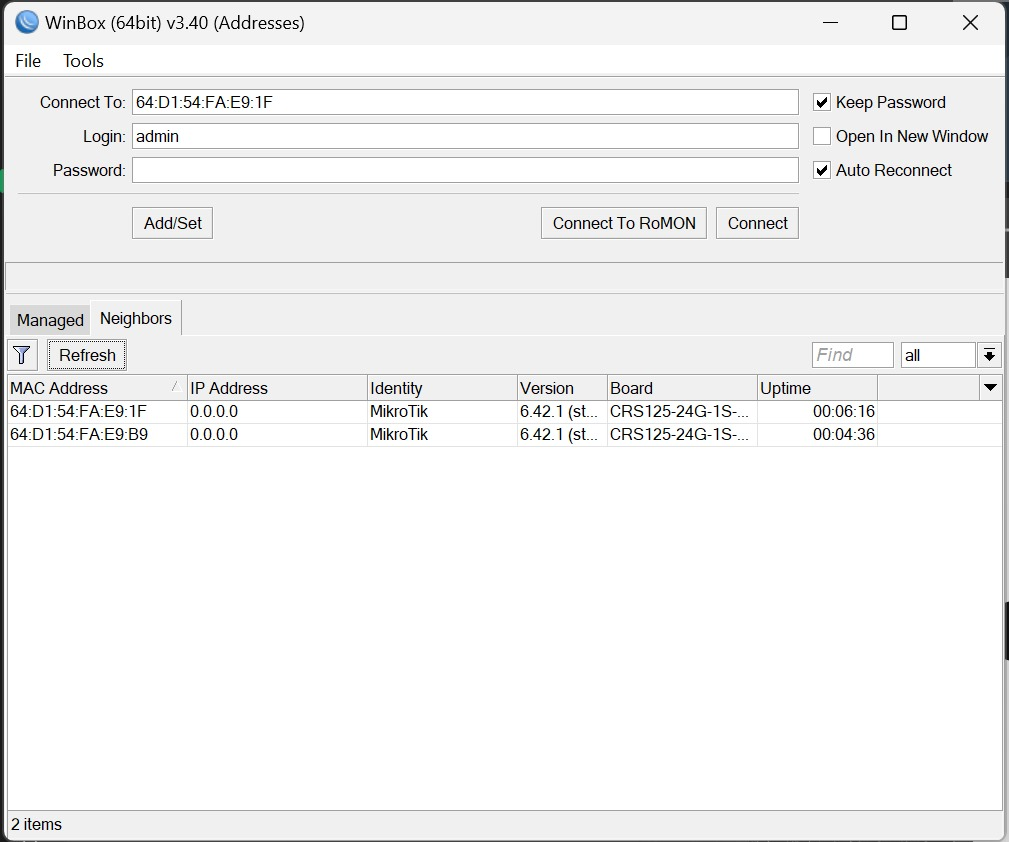
\includegraphics[width=0.7\linewidth]{P4/img/step1.jpg}
		\caption{Step 1}
		\label{fig:gambar1}
	\end{figure}

	% poin 2
	\item Jadikan Router menjadi DHCP Client agar bisa mendapat IP address dari Internet ITS. IP >
	Klik DHCP Client > Tambahkan DHCP Client > Pilih interface yang terhubung dengan Internet
	(ether2)> Klik Apply > Klik OK. Kita bisa memastikan koneksi ke internet dengan cara melakukan
	tes ping ke alamat IP 8.8.8.8
	
	\begin{figure}[H]
		\centering
		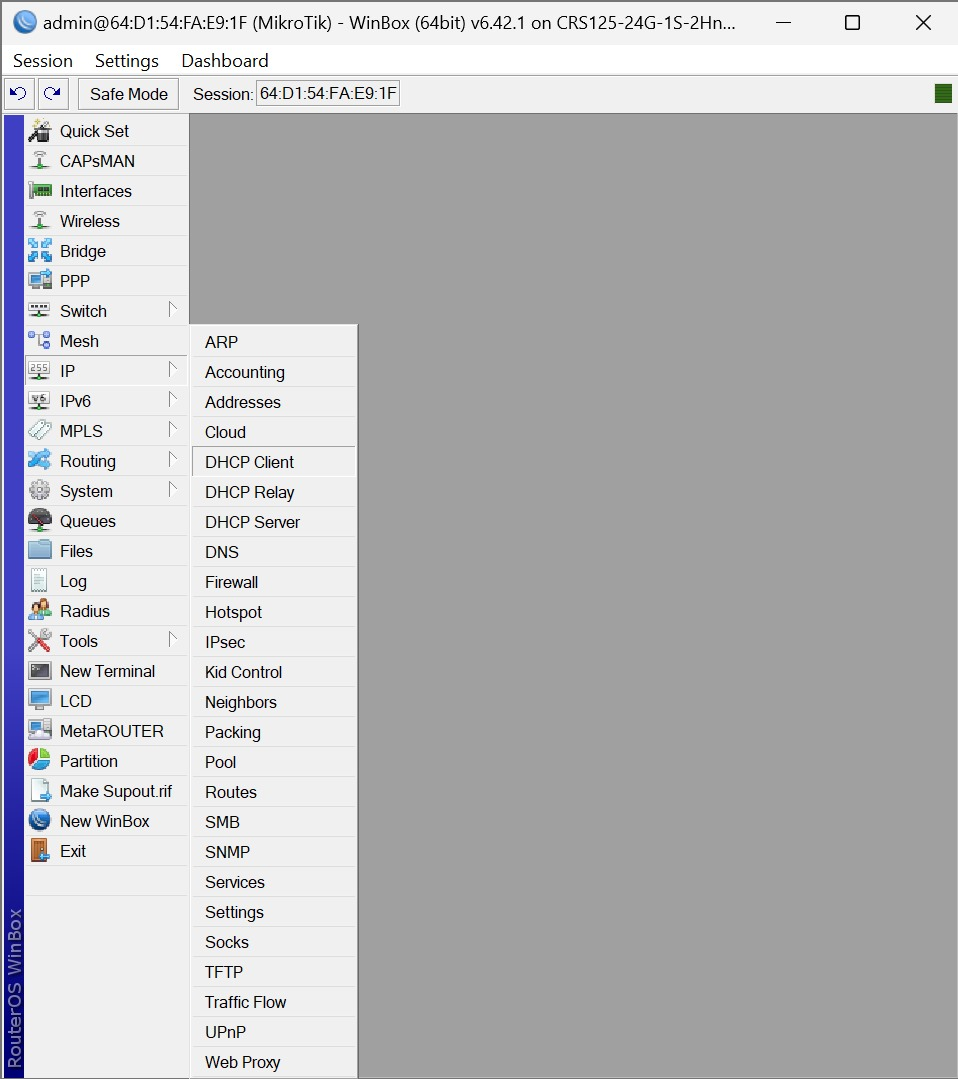
\includegraphics[width=0.5\linewidth]{P4/img/step2.1.jpg}
		\caption{Step 2.1}
		\label{fig:gambar2}
		
		\centering
		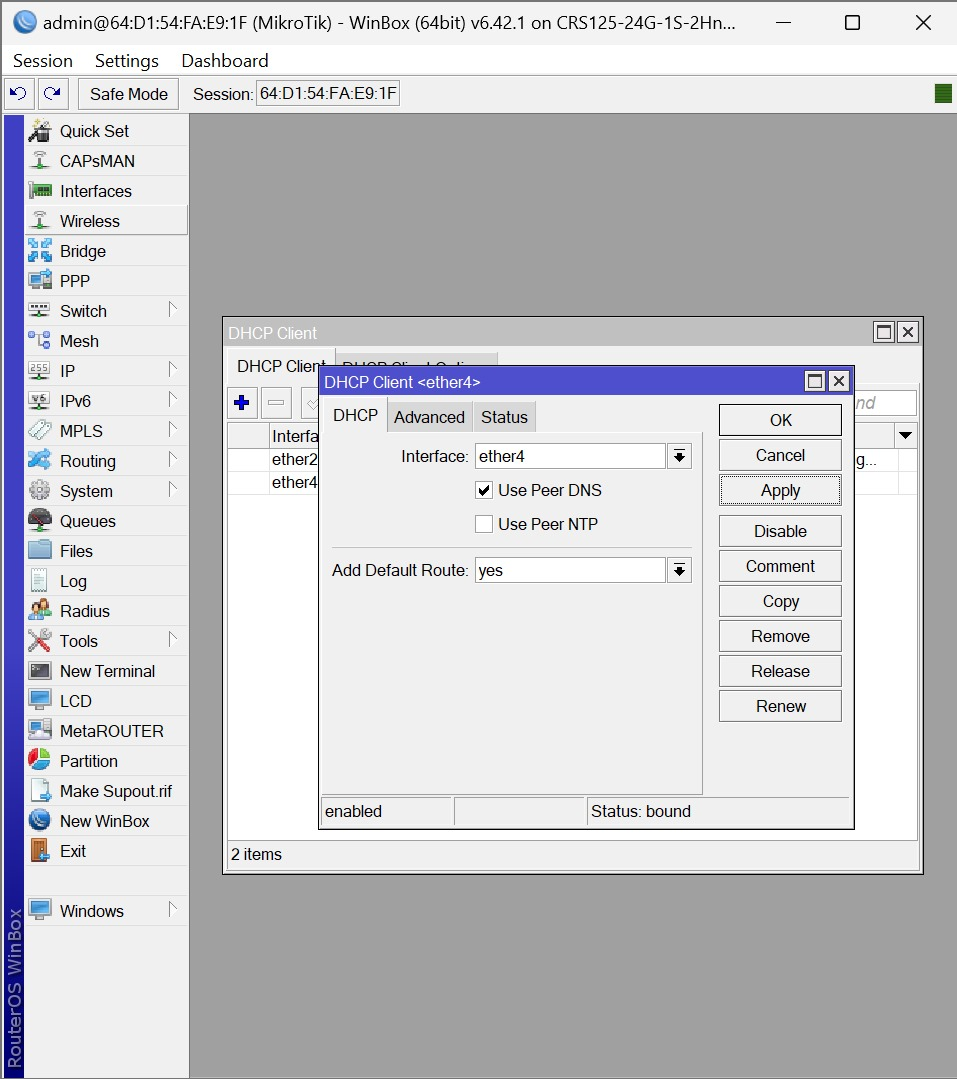
\includegraphics[width=0.5\linewidth]{P4/img/step2.2.jpg}
		\caption{Step 2.2}
		\label{fig:gambar2}
	\end{figure}

	% poin 3
	\item Buat IP address baru pada Router 1 untuk menghubungkan PC 1 dengan Router 1. Tambahkan
	IP address > Isi address > Pilih Interface yang terhubung ke PC (ether4) > Klik Apply > Klik OK.
	
	\begin{figure}[H]
		\centering
		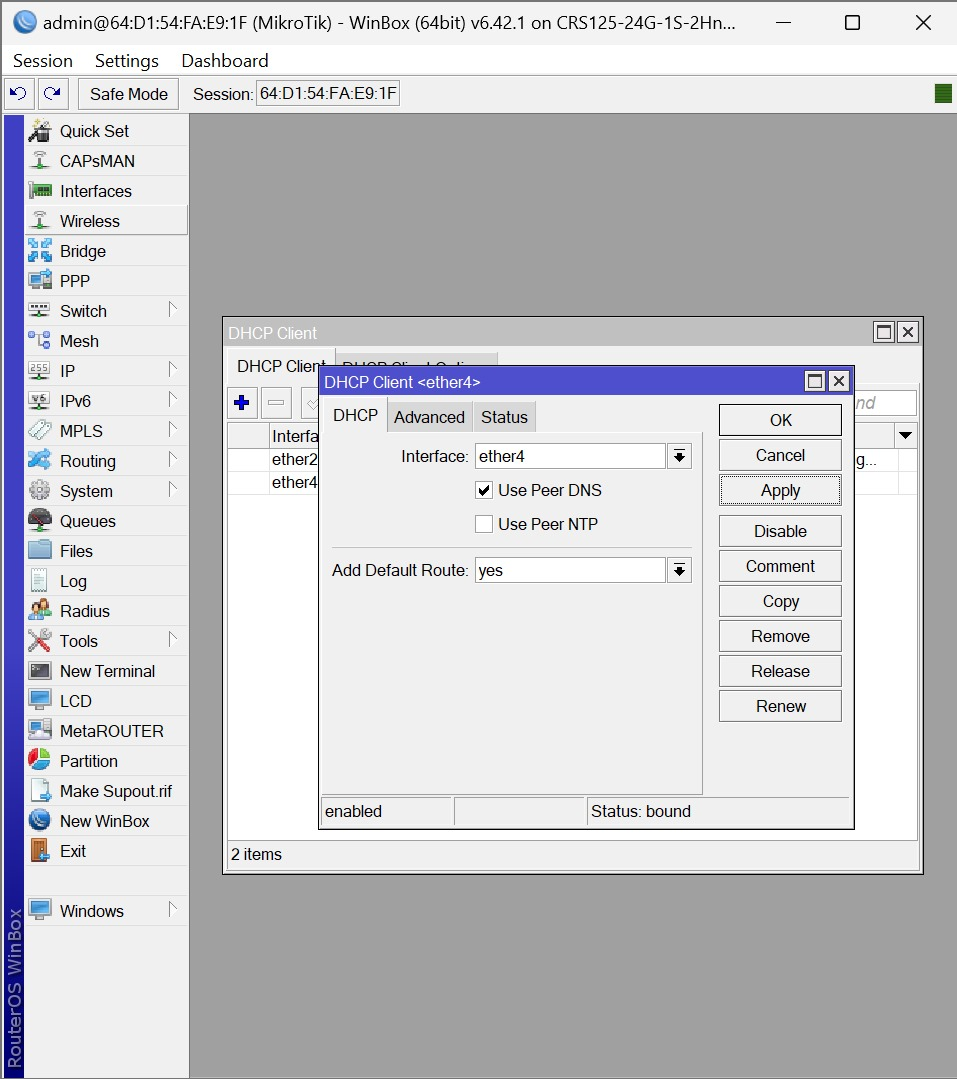
\includegraphics[width=0.5\linewidth]{P4/img/step3.jpg}
		\caption{Step 1}
		\label{fig:gambar1}
	\end{figure}

	% poin 4
	\item Atur IP pada PC 1 dengan mengubah pengaturan pada setting ethernet. Ubah IP perangkat
	yang otomatis menjadi manual, pastikan IP PC 1 masih satu jaringan dengan IP lokal yang
	diinginkan, isi Gateway dengan IP address Router 1 yang tersambung dengan PC 1. Berikan
	IP address yang berbeda dengan contoh yang ada di modul.
	
	\begin{figure}[H]
		\centering
		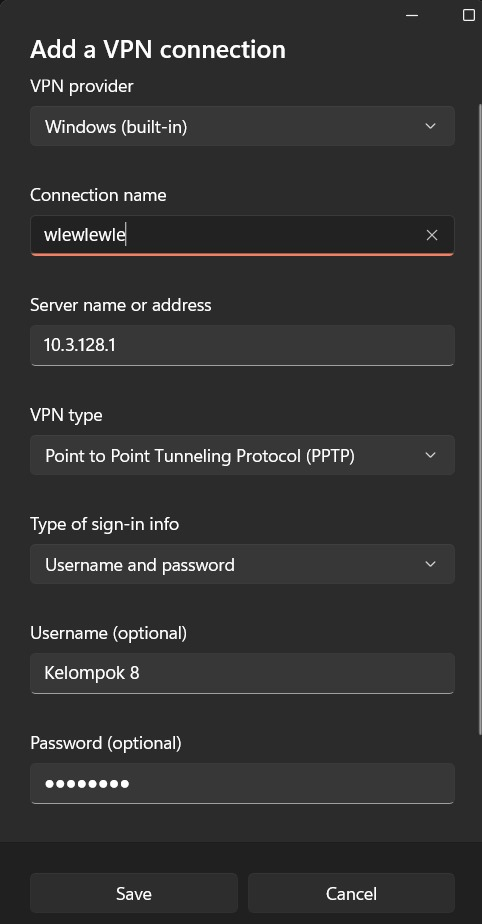
\includegraphics[width=0.5\linewidth]{P4/img/step4.jpg}
		\caption{Step 1}
		\label{fig:gambar1}
	\end{figure}

	% poin 5
	\item Buat PPTP untuk client pada tab Secret, dengan konfigurasi Nama “PPTP”, Password “123456”,
	Service “pptp”, Profile “default”. Local Address adalah IP address tunnel pada sisi server, diisi dengan “10.10.10.2”. 
	Remote Address adalah IP yang akan Client dapatkan, diisi dengan
	“10.10.10.3”. Pastikan Local Address dan Remote Address berada pada satu jaringan yang
	sama.
	
	\begin{figure}[H]
		\centering
		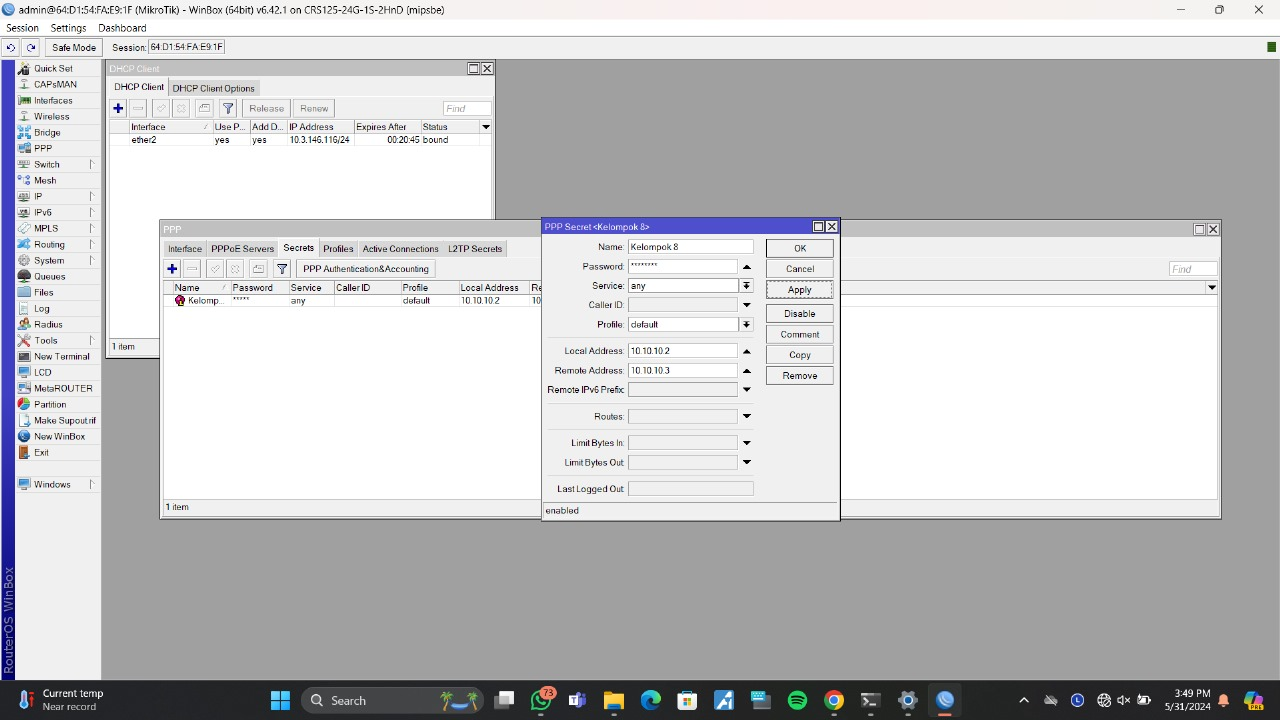
\includegraphics[width=0.5\linewidth]{P4/img/step5.jpg}
		\caption{Step 1}
		\label{fig:gambar1}
	\end{figure}

	% poin 6
	\item Lakukan tes ping ke alamat Remote Address Router 2 untuk memastikan kedua Router sudah
	terhubung. 	
	
	\begin{figure}[H]
		\centering
		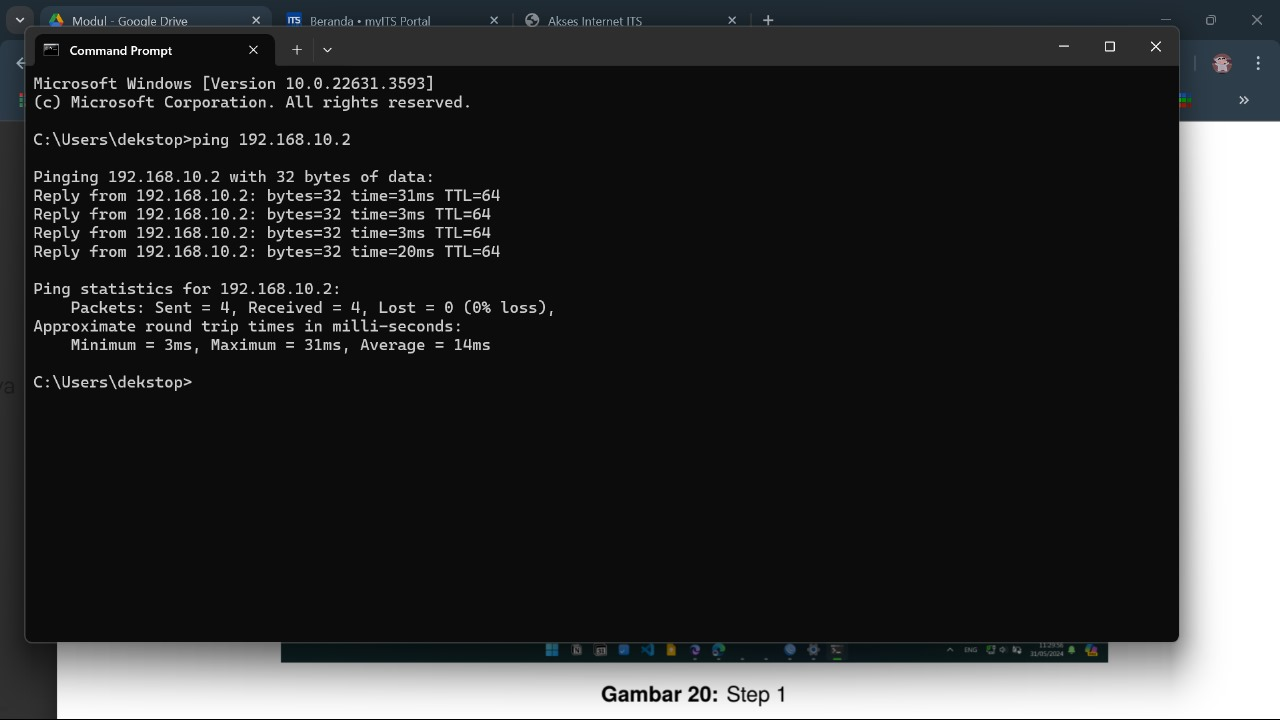
\includegraphics[width=0.5\linewidth]{P4/img/step6.jpg}
		\caption{Step 1}
		\label{fig:gambar1}
	\end{figure}

	% poin 7
	\item Lakukan routing statis agar kedua PC dapat berkomunikasi. Buka pada tab IP > Routes, lalu
	tambahkan jaringan. Masukkan alamat jaringan yang ingin dituju, melalui alamat Gateway pada
	router 2
	
	\begin{figure}[H]
		\centering
		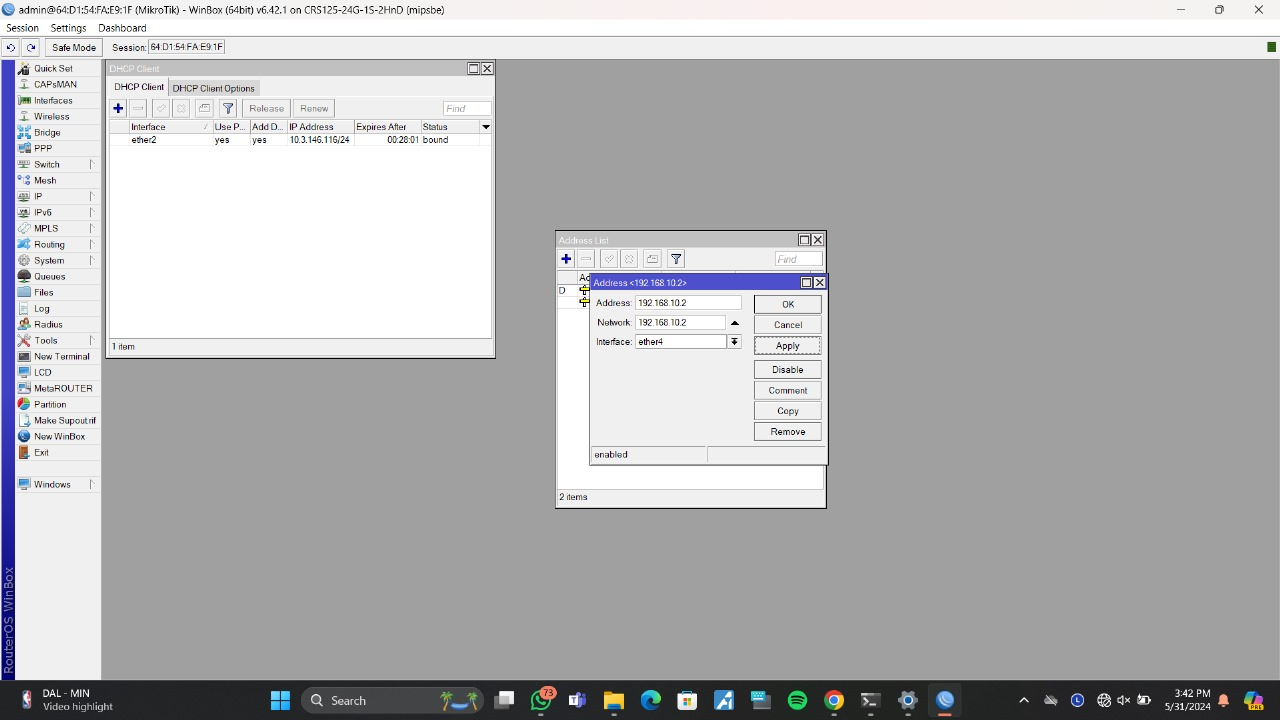
\includegraphics[width=0.5\linewidth]{P4/img/step7.jpg}
		\caption{Step 1}
		\label{fig:gambar1}
	\end{figure}

	% poin 8
	\item Lakukan tes ping ke ke PC 2 untuk memastikan kedua PC sudah terhubung.
	
	\begin{figure}[H]
		\centering
		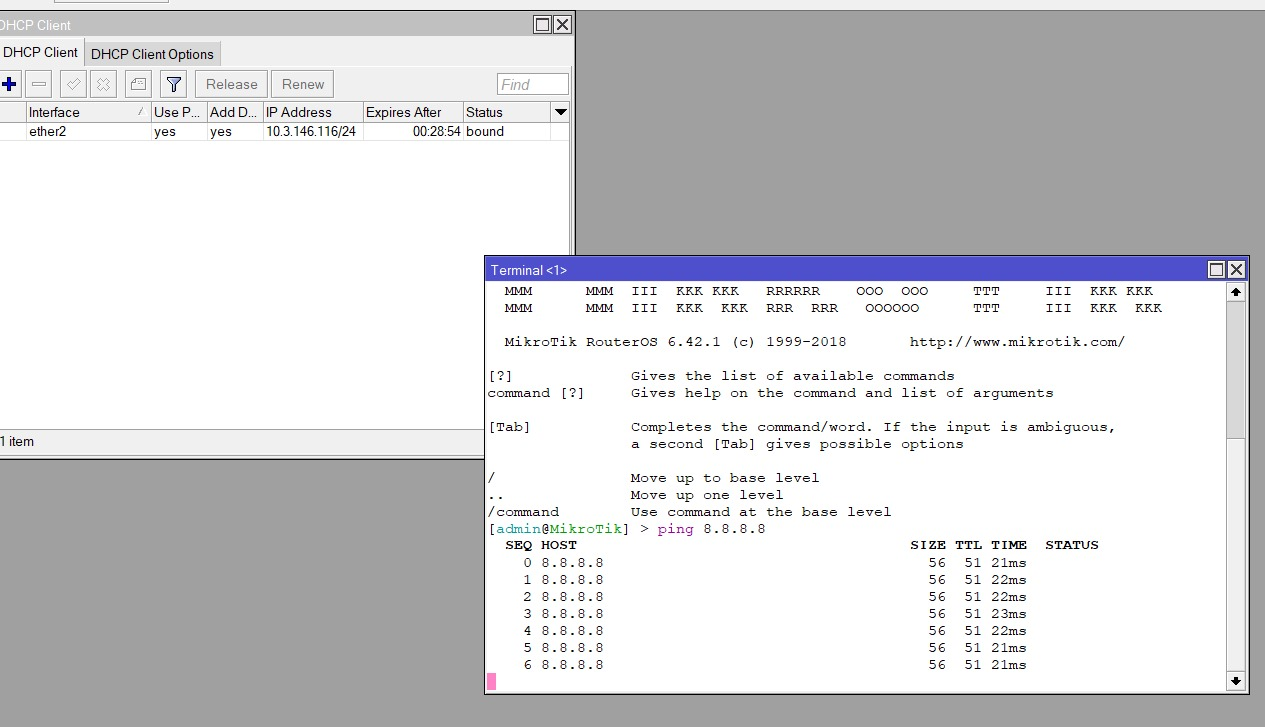
\includegraphics[width=0.5\linewidth]{P4/img/step8.jpg}
		\caption{Step 1}
		\label{fig:gambar1}
	\end{figure}

\end{enumerate}

%Langkah untuk konfigurasi Router 1
\begin{center} 
	\textbf{Konfigurasi PC 2}
\end{center}

\begin{enumerate}
	% poin 1
	\item Buka aplikasi Winbox pada PC dan lakukan hubungkan ke Router. Pastikan Login terisi “admin”,
	Klik Neighbors > Klik Refresh > Pilih Router yang ingin disambungkan > Klik Connect.
	
	\begin{figure}[H]
		\centering
		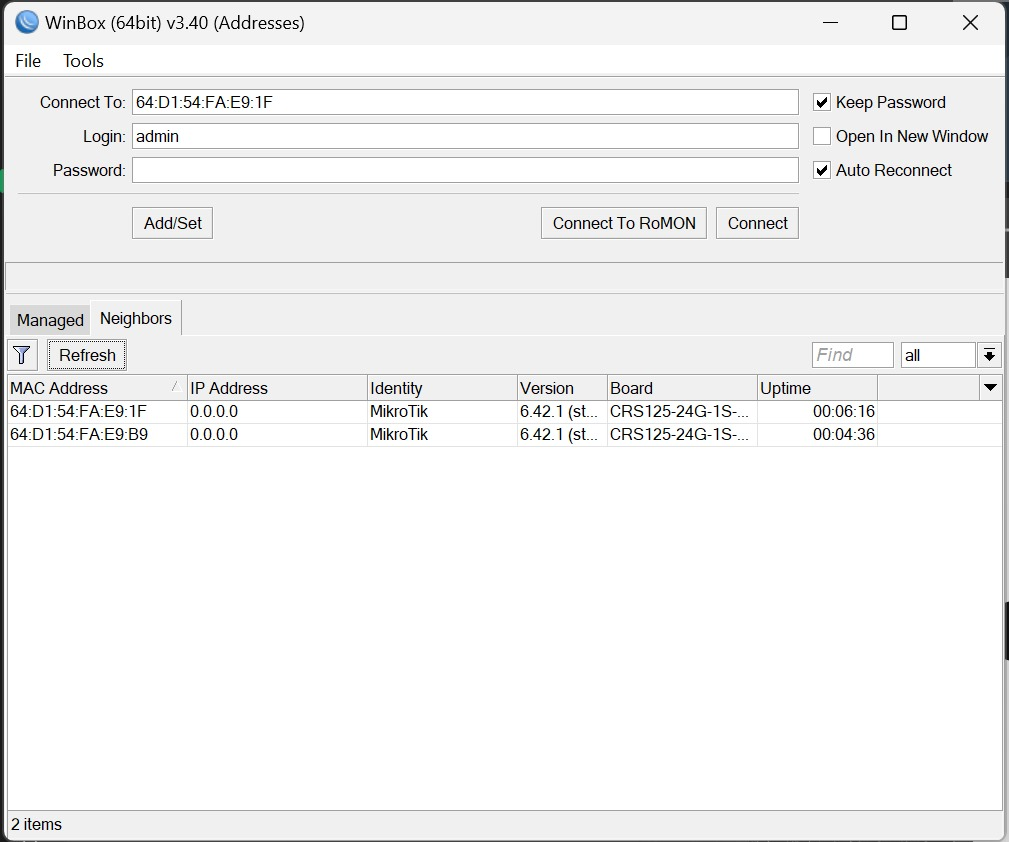
\includegraphics[width=0.5\linewidth]{P4/img/2step1.jpg}
		\caption{Step 1}
		\label{fig:gambar1}
	\end{figure}

	% poin 2
	\item Jadikan Router menjadi DHCP Client agar bisa mendapat IP address dari Internet ITS. IP >
	Klik DHCP Client > Tambahkan DHCP Client > Pilih interface yang terhubung dengan Internet
	(ether2)> Klik Apply > Klik OK. Kita bisa memastikan koneksi ke internet dengan cara melakukan
	tes ping ke alamat IP 8.8.8.8	
	
	\begin{figure}[H]
		\centering
		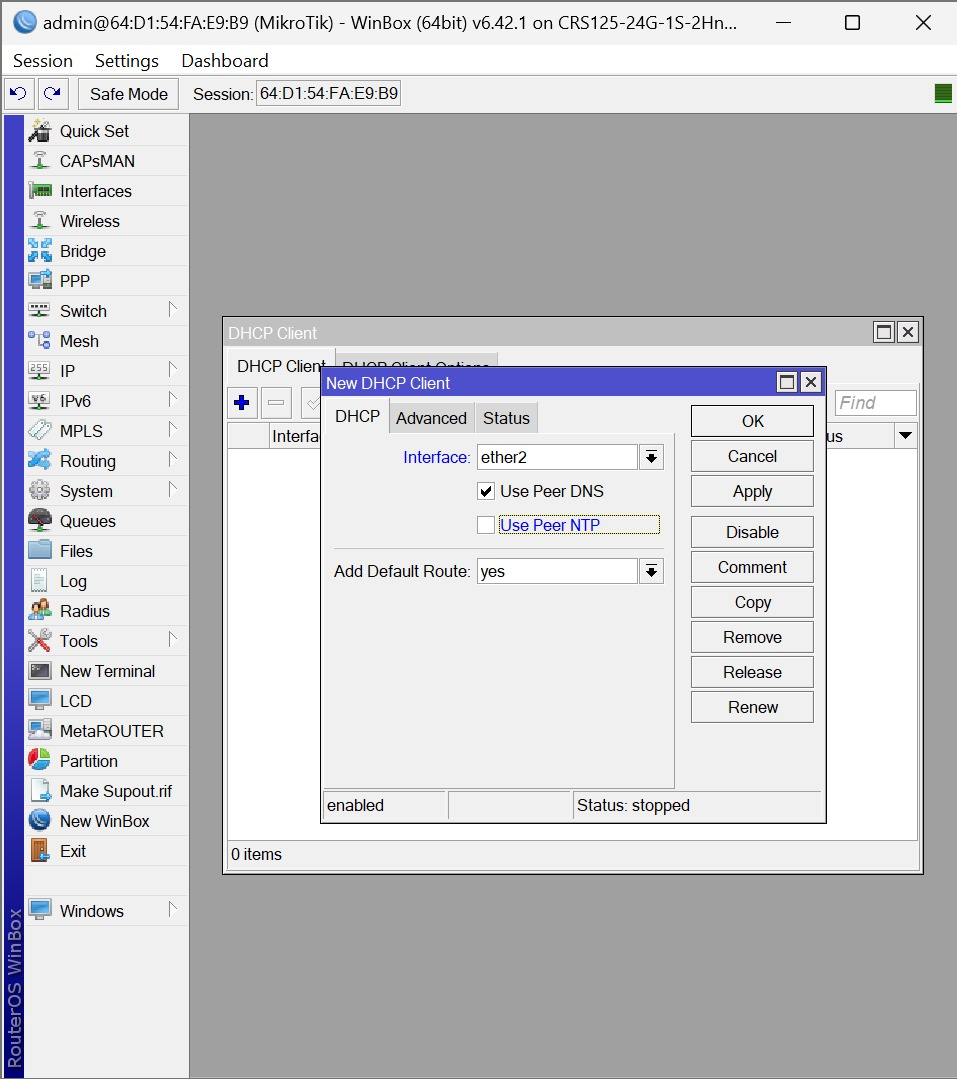
\includegraphics[width=0.5\linewidth]{P4/img/2step2.1.jpg}
		\caption{Step 2.1}
		\label{fig:gambar1}

		\centering
		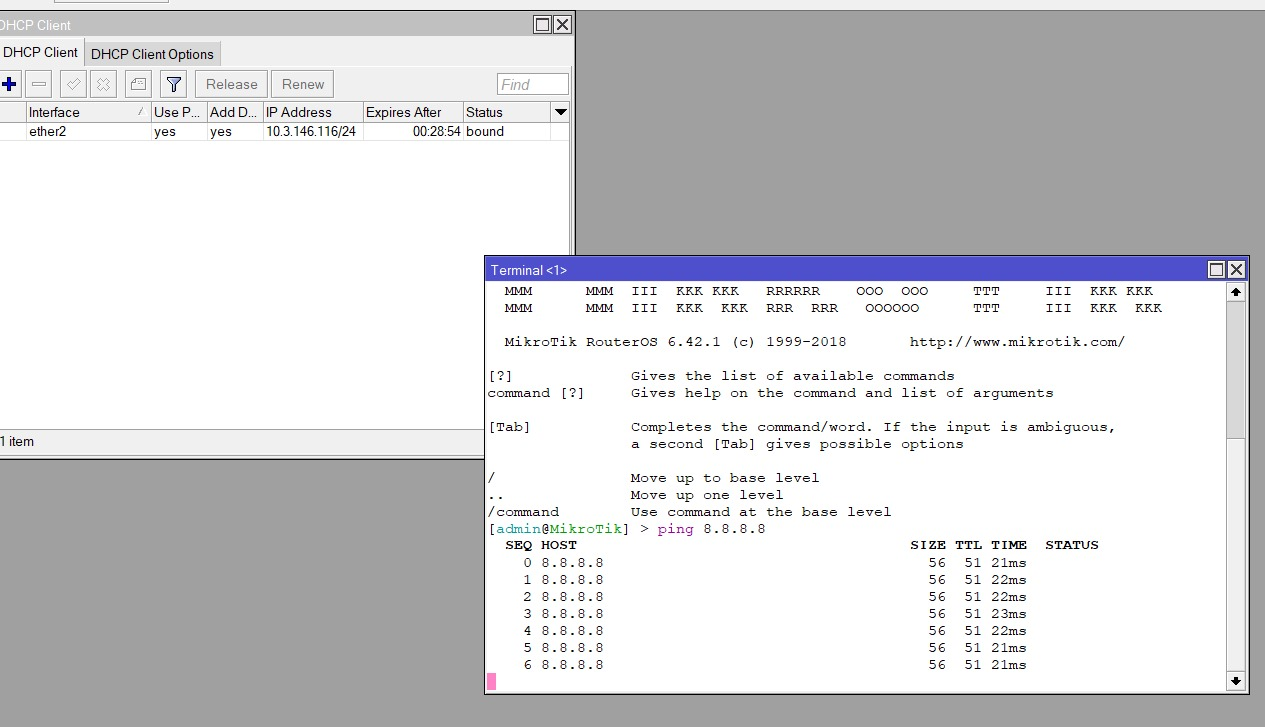
\includegraphics[width=0.5\linewidth]{P4/img/2step2.2.jpg}
		\caption{Step 2.2}
		\label{fig:gambar1}
	\end{figure}

	% poin 3
	\item Buat IP address baru pada Router 2 untuk menghubungkan PC 2 dengan Router 2. Tambahkan
	IP address > Isi address > Pilih Interface yang terhubung ke PC (ether4) > Klik Apply > Klik OK.
	
	\begin{figure}[H]
		\centering
		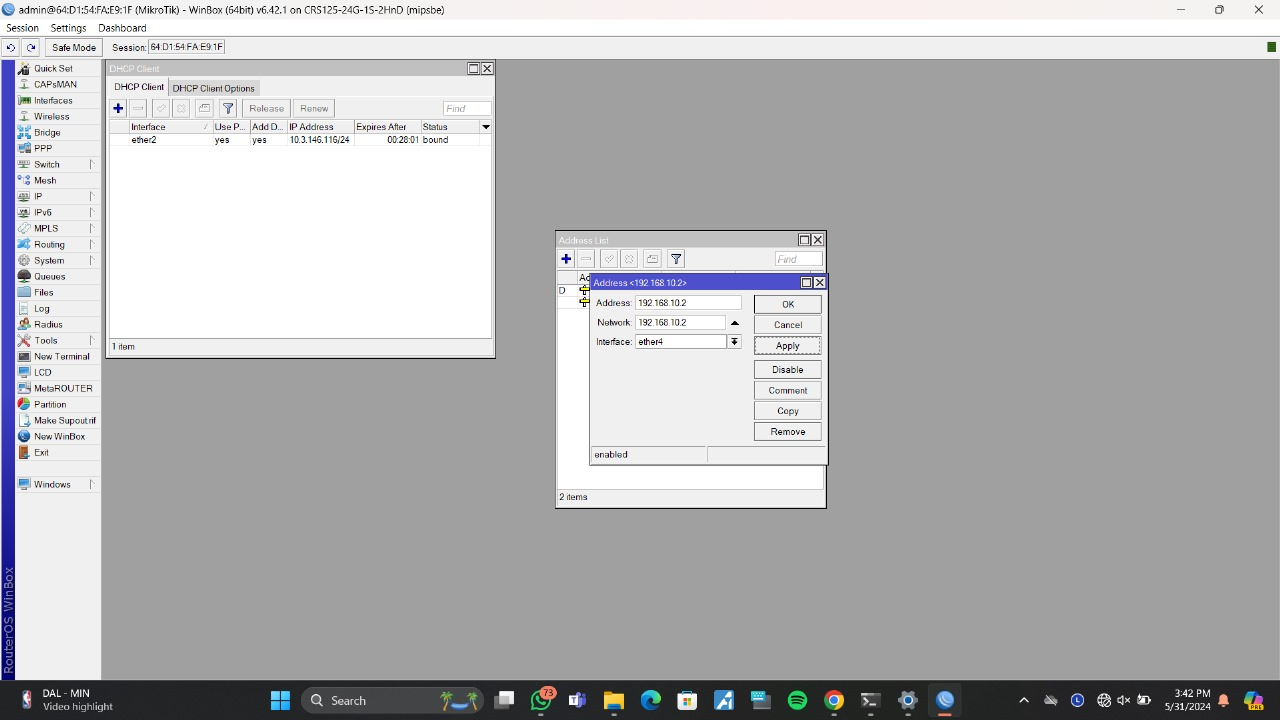
\includegraphics[width=0.5\linewidth]{P4/img/2step3.jpg}
		\caption{Step 1}
		\label{fig:gambar1}
	\end{figure}

	% poin 4
	\item Atur IP pada PC 2 dengan mengubah pengaturan pada setting ethernet. Ubah IP perangkat
	yang otomatis menjadi manual, pastikan IP PC 2 masih satu jaringan dengan IP lokal yang
	diinginkan, isi Gateway dengan IP address Router 2 yang tersambung dengan PC 2. Berikan
	IP address yang berbeda dengan contoh yang ada di modul.
	
	\begin{figure}[H]
		\centering
		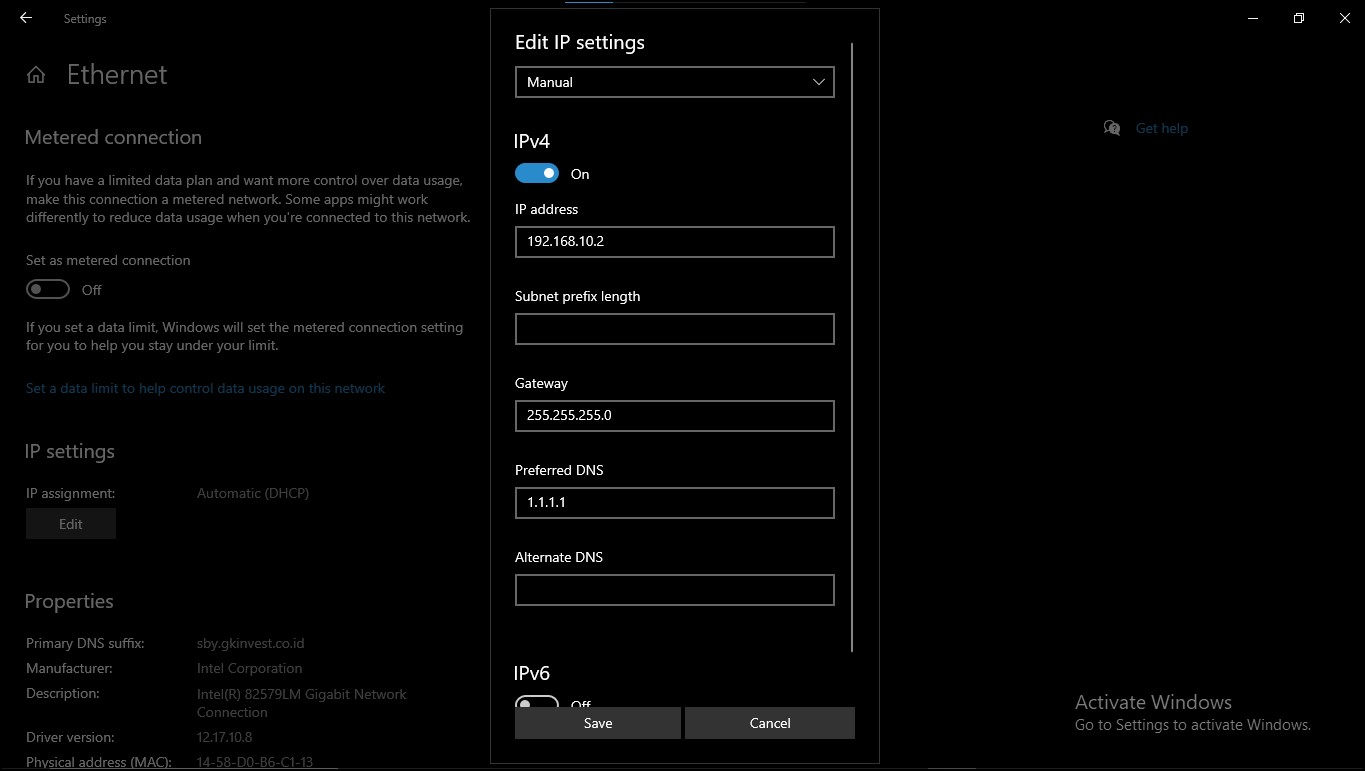
\includegraphics[width=0.5\linewidth]{P4/img/2step4.jpg}
		\caption{Step 1}
		\label{fig:gambar1}
	\end{figure}

	% poin 5
	\item Hubungkan client PPTP dengan server PPTP, untuk melakukan hal tersebut, buatlah PPTP
	Client baru kemudian konfigurasi koneksi pada tab Dial Out, dengan konfigurasi Connect To
	“10.3.142.134”, Connect To adalah IP address pada Router 1 yang terhubung ke internet. konfigurasi Nama “PPTP”, Password “123456”, Profile “default-encryption”. Pastikan Nama dan
	Password sesuai dengan yang sudah di buat.
	
	\begin{figure}[H]
		\centering
		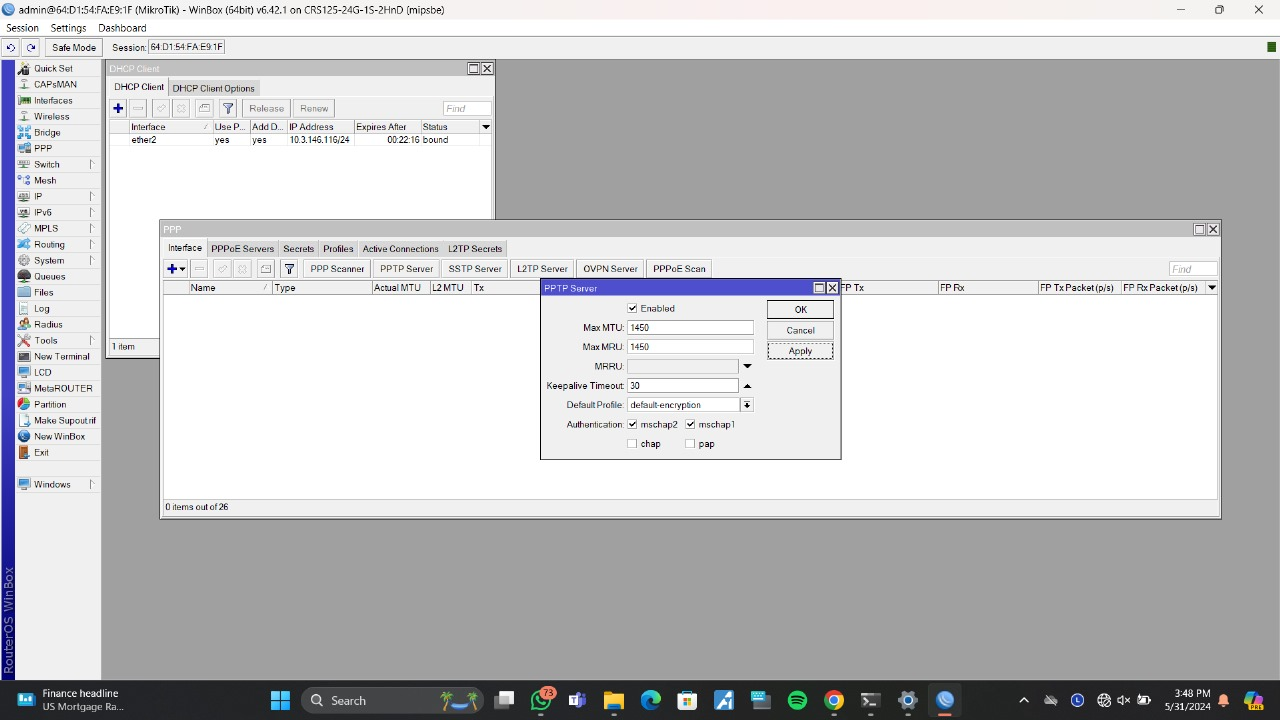
\includegraphics[width=0.5\linewidth]{P4/img/2step5.jpg}
		\caption{Step 1}
		\label{fig:gambar1}
	\end{figure}

	% poin 6
	\item Lakukan tes ping ke alamat Local Address Router 1 untuk memastikan kedua Router sudah
	terhubung.
	
	\begin{figure}[H]
		\centering
		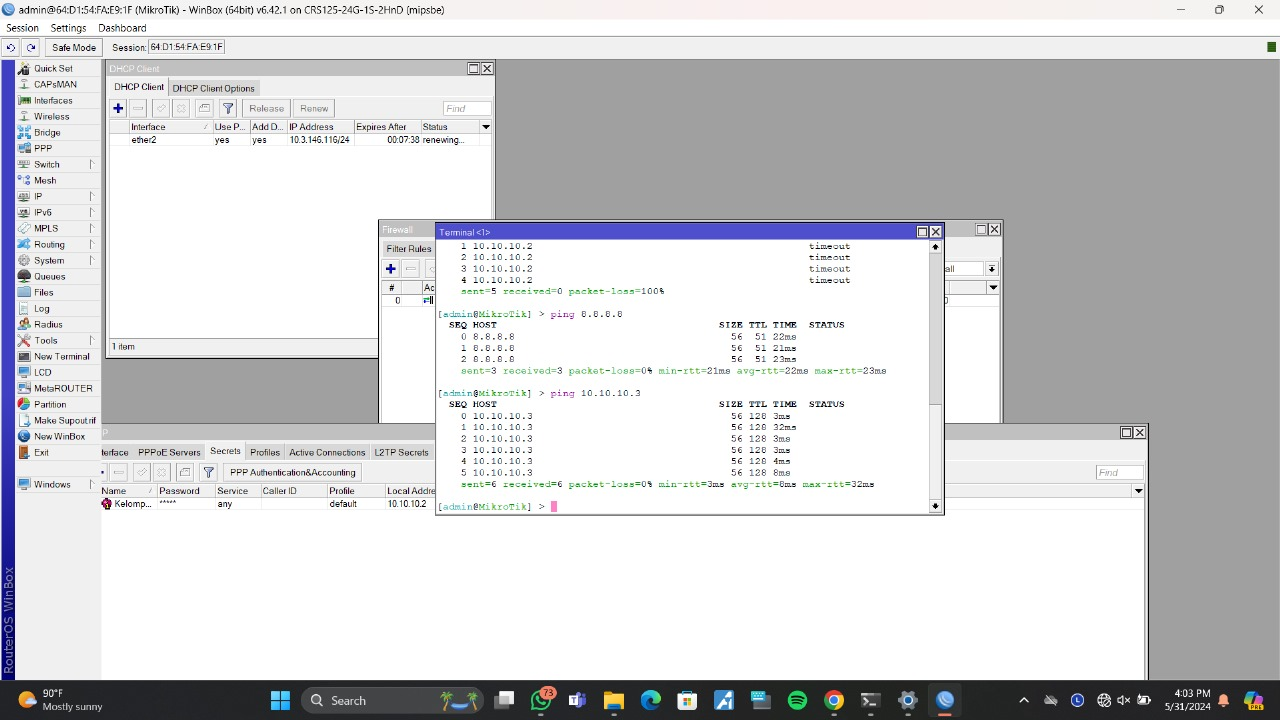
\includegraphics[width=0.5\linewidth]{P4/img/2step6.jpg}
		\caption{Step 1}
		\label{fig:gambar1}
	\end{figure}

	% poin 7
	\item Lakukan routing statis agar kedua PC dapat berkomunikasi. Buka pada tab IP > Routes, lalu
	tambahkan jaringan. Masukkan alamat jaringan yang ingin dituju, melalui alamat Gateway pada
	router 2
	
	\begin{figure}[H]
		\centering
		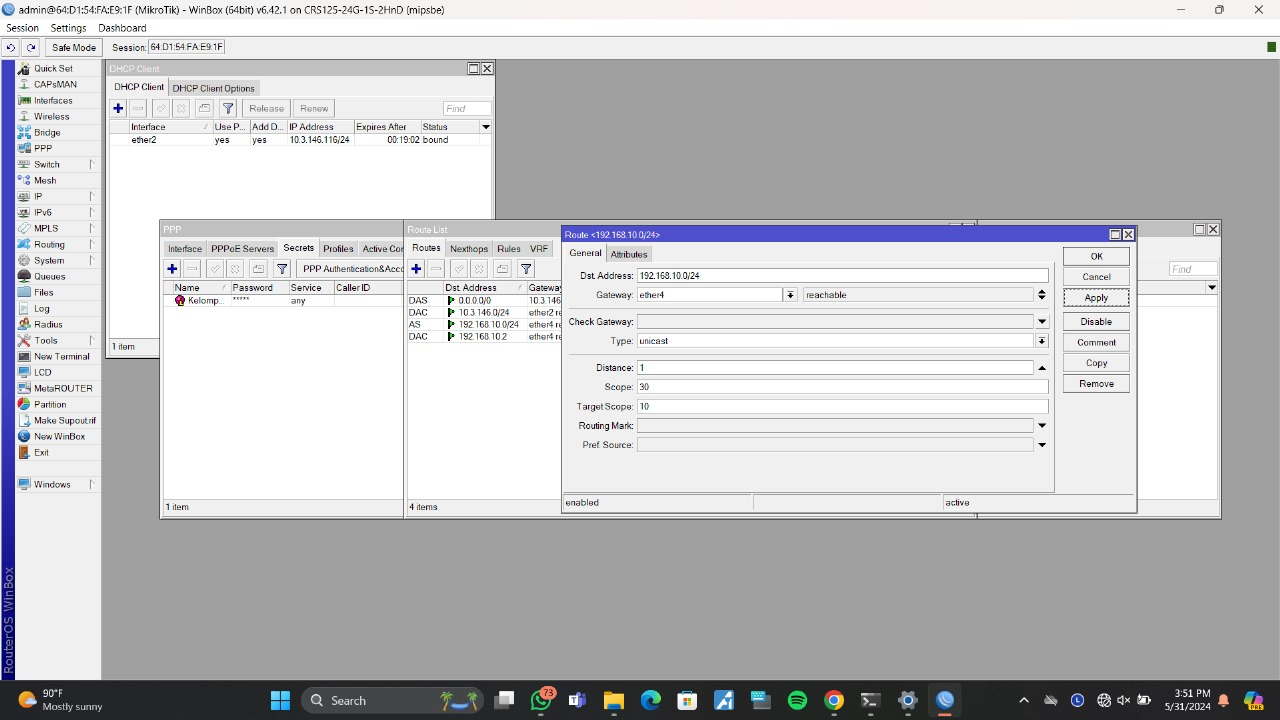
\includegraphics[width=0.5\linewidth]{P4/img/2step7.jpg}
		\caption{Step 1}
		\label{fig:gambar1}
	\end{figure}

	% poin 8
	\item Lakukan tes ping ke ke PC 1 untuk memastikan kedua PC sudah terhubung.
	
	\begin{figure}[H]
		\centering
		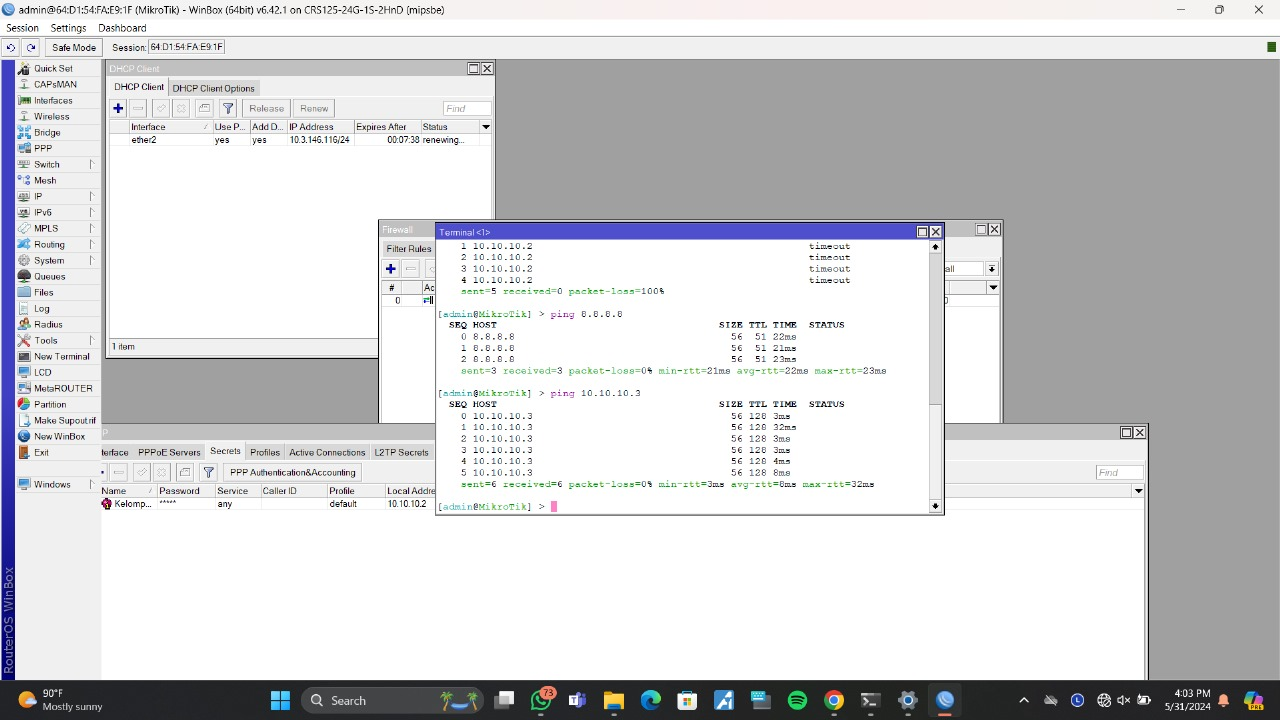
\includegraphics[width=0.5\linewidth]{P4/img/2step6.jpg}
		\caption{Step 1}
		\label{fig:gambar1}
	\end{figure}

\end{enumerate}


\section{Hasil Percobaan}
akan diisi setelah praktikum
%===========================================================%

\section{Kesimpulan}
akan diisi setelah praktikum
%===========================================================%

\section{Lampiran}

\subsection{Tugas Pendahuluan}
\begin{enumerate}
	\item Apa itu PPTP dan bagaimana cara kerjanya?
	\\ \indent PPTP (Point-to-Point Tunneling Protocol) adalah sebuah protokol jaringan yang memungkinkan penggunaan jaringan virtual (VPN) untuk menghubungkan perangkat yang berbeda melalui jaringan publik yang tidak aman. 
	PPTP bekerja dengan cara mengenkripsi, menegosiasi, serta mengotentifikasi setiap data yang dikirimkan melalui jaringan. 
	\\ cara kerja PPTP kurang lebih seperti berikut:
	\begin{itemize}
		\item Mengenkripsi Data: PPTP mengenkripsi data yang dikirimkan melalui jaringan menggunakan MPPE-128 bit enkripsi.
		\item Mengotentikasi: PPTP menggunakan Microsoft Challange/Replay Handshake Protocol version 2 (MS-CHAPv2) untuk otentikasi client ke server.
		\item Menegosiasi: PPTP menegosiasi PPP (Point-to-Point Protocol) untuk mengatur koneksi jaringan dan mengenkripsi data yang dikirimkan.
		\item Membuat Tunnel: PPTP membuat sebuah tunnel VPN yang memungkinkan data dikirimkan melalui jaringan publik yang tidak aman tanpa terpengaruh oleh gangguan luar
	\end{itemize}

	\item Apa kelebihan dan kekurangan dari penggunaan PPTP dibandingkan protokol VPN lainnya seperti L2TP atau OpenVPN?
	
	\begin{itemize}
		\item Kelebihan :
		\begin{itemize}
			\item[\ding{58}] Kemudahan Konfigurasi: \\ PPTP sangat mudah diatur dan diimplementasikan, sering kali hanya memerlukan nama pengguna, kata sandi, dan alamat server.
			\item[\ding{58}] Kompatibilitas Luas: \\ PPTP didukung oleh hampir semua sistem operasi dan perangkat, termasuk Windows, macOS, Linux, iOS, dan Android.
			\item[\ding{58}] Kecepatan: \\ Karena enkripsi yang lebih sederhana, PPTP cenderung lebih cepat dibandingkan dengan protokol VPN lainnya.
		\end{itemize}

		\item Kekurangan :
		\begin{itemize}
			\item[\ding{56}] Keamanan: \\ PPTP bukan VPN yang paling aman. PPTP dianggap kurang aman karena kelemahan dalam protokol MS-CHAP v2 yang digunakan untuk otentikasi. Ini membuatnya rentan terhadap serangan brute-force dan penyadapan.
			\item[\ding{56}] Pemblokiran: \\ PPTP lebih mudah dideteksi dan diblokir oleh firewall dan ISP karena menggunakan port tetap (TCP port 1723) dan GRE (Generic Routing Encapsulation).
			\item[\ding{56}] Tidak Mempunyai Enkripsi yang Baik: \\ PPTP menggunakan MPPE-128 bit enkripsi, yang tidak sebaik enkripsi yang digunakan oleh protokol lain seperti L2TP dan OpenVPN.
		\end{itemize}
	\end{itemize}

\end{enumerate}

\subsection{Dokumentasi saat Praktikum}

\begin{figure}[H]
	\centering
	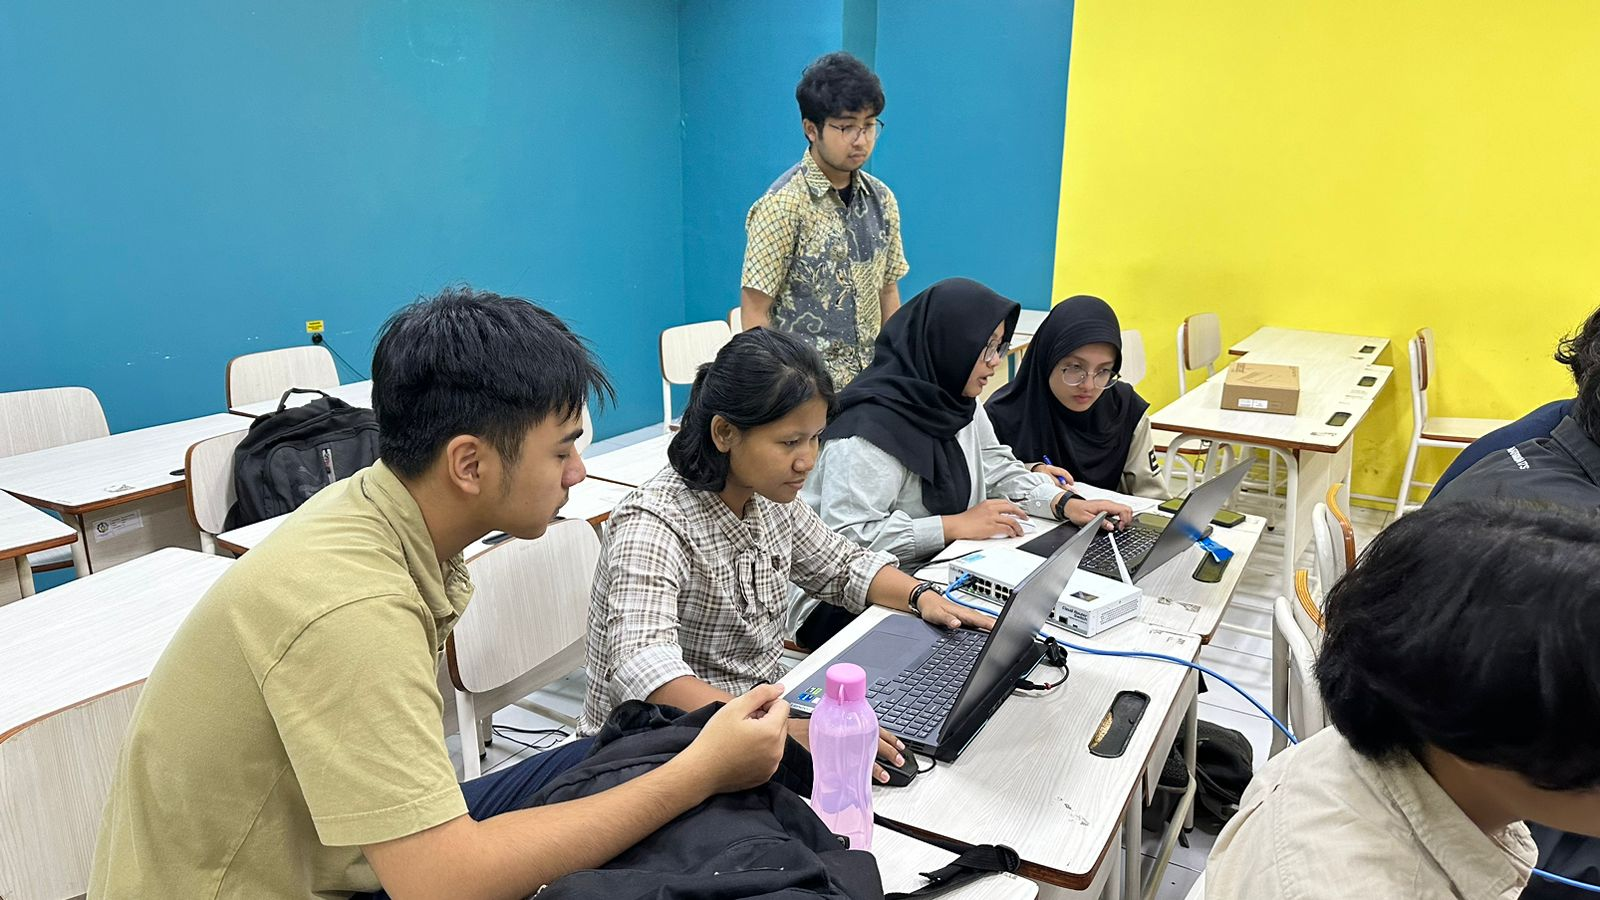
\includegraphics[width=0.75\linewidth]{P4/img/dokumpraktikum.jpg}
	\caption{Dokumentasi saat praktikum}
	\label{fig:gambar32}
\end{figure}